\documentclass[xcolor=dvipsnames]{beamer} % dvipsnames gives more built-in colors
\mode<presentation>

\usetheme{Boadilla}

\definecolor{GWdarkblue}{HTML}{033C5A}

\usecolortheme[named=GWdarkblue]{structure}

% Sets the font
\usepackage[defaultfam,tabular,lining]{montserrat}
\setbeamerfont{title}{shape=\scshape}
\setbeamerfont{frametitle}{shape=\scshape}
%Remove "Figure" from captions
\setbeamertemplate{caption}{\raggedright\insertcaption\par}

\usepackage{graphicx}
\usepackage{tabularx}
\usepackage{hyperref}

\title[Researcher Choices and Bias]{Researcher Choices and Bias}
\author[SMPA 2152]{Data Analysis for Journalism and Political Communication (Fall 2024)}
\date{Prof. Bell}

\begin{document}

%%%%%%%%%%%%%%%%%%%%%%%%%%%%%%%%%%%%%%%%%%%%%%%%%%%%%%%%%%%%%%%%%%
\frame{
\titlepage
}

%%%%%%%%%%%%%%%%%%%%%%%%%%%%%%%%%%%%%%%%%%%%%%%%%%%%%%%%%%%%%%%%%%
\frame{

\begin{center}
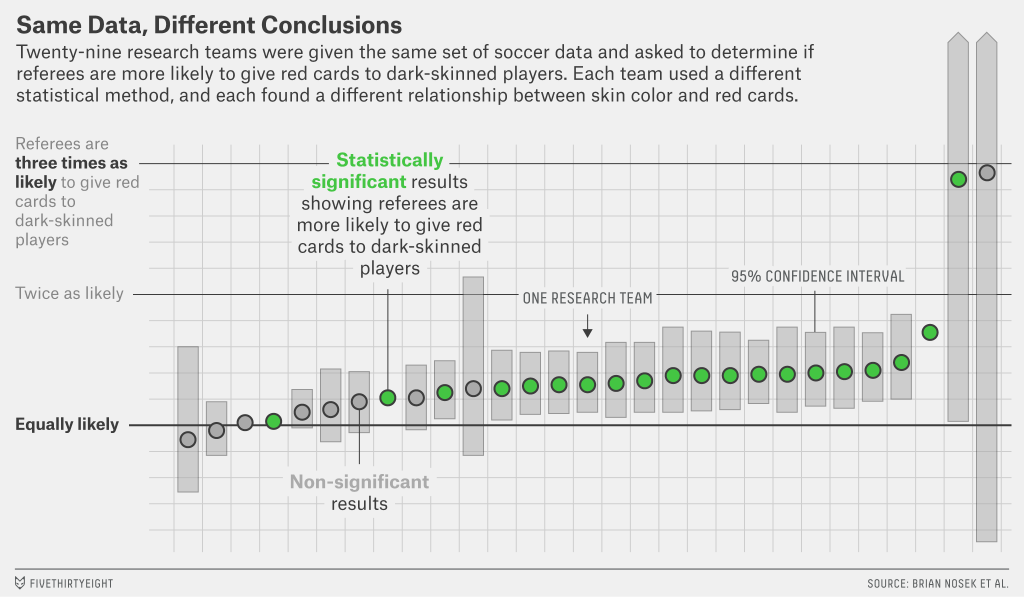
\includegraphics[width=.9\textwidth]{soccer_same_data_different_results.png}
\end{center}
}

%%%%%%%%%%%%%%%%%%%%%%%%%%%%%%%%%%%%%%%%%%%%%%%%%%%%%%%%%%%%%%%%%%
\frame{\frametitle{Researcher Choices}

\begin{enumerate}[<+->]
    \item What is my hypothesis?
    \item What do I measure?
    \item How do I collect my data?
    \item How much data do I collect?
    \item What statistical analyses do I use?
    \item How do I handle outliers, missing data, and other peculiarities?
\end{enumerate}
}

%%%%%%%%%%%%%%%%%%%%%%%%%%%%%%%%%%%%%%%%%%%%%%%%%%%%%%%%%%%%%%%%%%
\frame{\frametitle{What is my hypothesis?}

Choosing a hypothesis is all about avoiding error:\\~\\

\begin{itemize}[<+->]
    \item \textbf{Type I error}: False positives
    \begin{itemize}
        \item<.-> Sending the innocent to jail - this is bad!\\~\\
    \end{itemize}
    \item \textbf{Type II error}: False negatives
    \begin{itemize}
        \item<.-> Letting the guilty go free - we can accept this
    \end{itemize}
\end{itemize}
~\\
\only<3->{Our goal is to reduce Type I error. Assume that the data is innocent (that the hypothesis is false) until it is proven guilty.}
}

%%%%%%%%%%%%%%%%%%%%%%%%%%%%%%%%%%%%%%%%%%%%%%%%%%%%%%%%%%%%%%%%%%
\frame{\frametitle{Measuring Type I Error}

\only<1-3>{
    \begin{block}{P-value}
    The chance that we would get a particular result from our test if the true answer is false
    \end{block}

    \begin{itemize}[<+(1)->]
        \item The p-value is our chance of committing a Type I error - sending the innocent to jail
        \item Common p-value cut-offs in scientific research: .01, .05, and .1 indicate \textbf{statistical significance}
    \end{itemize}
}
\only<4->{
    \textbf{Hypothesis:} A student cheated on an exam.
    ~\\
    ~\\
    \begin{itemize}
        \item<5-> The student performed much better on this exam than on previous exams
        \item<6-> The student finished their exam more quickly than other students
        \item<7-> The student's roommate saw them up all night studying before the exam
        \item<8-> The student missed the same questions as other students
    \end{itemize}
    ~\\
    \textbf{P-value (chance that we conclude that student cheated, but they did not):} \only<4>{.50}\only<5>{.25}\only<6>{.15}\only<7>{.40}\only<8>{.75}
}
}
%%%%%%%%%%%%%%%%%%%%%%%%%%%%%%%%%%%%%%%%%%%%%%%%%%%%%%%%%%%%%%%%%%
\frame{\frametitle{The Scientific Method}

\begin{itemize}[<+->]
    \item P-values are a product of the data we use and our choices about what we include and exclude from the analysis.
    \item We follow the scientific method: Theory $\Rightarrow$ Hypothesis $\Rightarrow$ Test $\Rightarrow$ Analyze $\Rightarrow$ Report
    \item But in practice, no analysis plan survives contact with the data
\end{itemize}
}

%%%%%%%%%%%%%%%%%%%%%%%%%%%%%%%%%%%%%%%%%%%%%%%%%%%%%%%%%%%%%%%%%%
\frame{\frametitle{Are Democrats or Republicans Good for the Economy?}

Use FiveThirtyEight's online modeling tool to test what you think is the best approach to answering the question. There are no right or wrong answers - just select the model you think is best, and report your results in the form:

\begin{center}
\href{https://bit.ly/smpa2152}{https://bit.ly/smpa2152}\\
~\\

\includegraphics[height=.3\textheight]{bit.ly_smpa2152.png}
\end{center}

(The link to the tool is on the form.)
}


%%%%%%%%%%%%%%%%%%%%%%%%%%%%%%%%%%%%%%%%%%%%%%%%%%%%%%%%%%%%%%%%%%
\frame{\frametitle{Misuses of P-values}

\begin{itemize}[<+->]
    \item \textbf{P-hacking}: Manipulating data or analysis in order to find a statistically significant result
    \item \textbf{HARKing}: \textbf{H}ypothesizing \textbf{a}fter \textbf{r}esults are \textbf{k}nown
    \item \textbf{File drawer bias/publication bias}: Only publishing statistically significant results
    \item Confusing statistical significance with substantive significance
\end{itemize}
}

%%%%%%%%%%%%%%%%%%%%%%%%%%%%%%%%%%%%%%%%%%%%%%%%%%%%%%%%%%%%%%%%%%
\frame{\frametitle{What do I measure?}

\begin{block}{Operationalization}
    The process of defining a measurable version of a concept
\end{block}
~\\
\only<2>{Suppose you were interested in measuring ``study quality,'' a variable indicating how well a student studies. What are some ways you would measure this concept?}
\only<3->{
\begin{itemize}[<+(2)->]
    \item Principles of good operationalization:
    \begin{enumerate}
        \item<.-> Unambiguous
        \item Concise
        \item Familiar
        \item Available
    \end{enumerate}
\end{itemize}
}
}

%%%%%%%%%%%%%%%%%%%%%%%%%%%%%%%%%%%%%%%%%%%%%%%%%%%%%%%%%%%%%%%%%%
\frame{\frametitle{Exercise: Operationalization}

\begin{enumerate}
    \item You want to measure \href{https://worldhappiness.report/}{how happy people are}
    \item You want to measure \href{https://www.dmv.virginia.gov/sites/default/files/forms/csma19.pdf}{people's driving ability}
    \item You want to measure the \href{https://voteview.com/congress/house}{political ideology of a member of Congress}
\end{enumerate}
}

%%%%%%%%%%%%%%%%%%%%%%%%%%%%%%%%%%%%%%%%%%%%%%%%%%%%%%%%%%%%%%%%%%
\frame{\frametitle{How do I collect my data?}

\begin{block}{Data Generating Process}
    The rules and procedures that produce the data one is interested in
\end{block}

\begin{itemize}[<+(1)->]
    \item No amount of statistical wizardry can compensate for bad data
    \item The gold standard of data generating processes is the \textbf{random sample}
\end{itemize}

\centering
\vspace{1em}
\only<2>{
    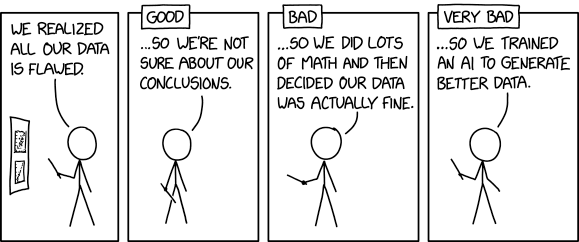
\includegraphics[width=.6\textwidth]{dgp_xkcd.png}
    }
}

%%%%%%%%%%%%%%%%%%%%%%%%%%%%%%%%%%%%%%%%%%%%%%%%%%%%%%%%%%%%%%%%%%
\frame{\frametitle{Sampling}
\begin{itemize}[<+->]
    \item The group we are interested in studying is known as the \textbf{population}
    \item Often, we are not able to count every unit in the population, so we take a \textbf{sample}
    \item The key to any data analysis project is a quality sample, which is determined by two elements:
    \begin{enumerate}
        \item A \textbf{random sample} of the population
        \item The \textbf{sample size} is sufficiently large
    \end{enumerate}
\end{itemize}
}

%%%%%%%%%%%%%%%%%%%%%%%%%%%%%%%%%%%%%%%%%%%%%%%%%%%%%%%%%%%%%%%%%%
\frame{\frametitle{Random Sample}

\only<1-4>{\begin{block}{Definition}
    The probability of any given unit being drawn from the population is uniform (the same)
\end{block}
~\\
\begin{itemize}[<+(1)->]
    \item A failure of each unit to have a uniform probability of being drawn from the population is known as \textbf{selection bias}
    \item Units are ``selecting'' into our data because they are more observable than other units
    \item Selection bias reduces our \textbf{generalizability} to the population because the data is not representative of the population
\end{itemize}
}

\only<5-7>{
Can I randomly sample 10 students from this class to generalize to:
\begin{itemize}[<+(4)->]
    \item the population of GW students?
    \item the population of SMPA students?
    \item the population of Data Analysis students?
\end{itemize}
}
}

%%%%%%%%%%%%%%%%%%%%%%%%%%%%%%%%%%%%%%%%%%%%%%%%%%%%%%%%%%%%%%%%%%
\frame{\frametitle{Exercise: Selection Bias}

}

%%%%%%%%%%%%%%%%%%%%%%%%%%%%%%%%%%%%%%%%%%%%%%%%%%%%%%%%%%%%%%%%%%
\frame{\frametitle{Biases in Research}

\begin{enumerate}
    \item Confirmation bias
    \item Desirability bias
    \item Authority bias
    \item Availability bias
    \item Certainty bias
\end{enumerate}

}

%%%%%%%%%%%%%%%%%%%%%%%%%%%%%%%%%%%%%%%%%%%%%%%%%%%%%%%%%%%%%%%%%%
\frame{\frametitle{Confirmation Bias}

\begin{block}{}
We privilege evidence that supports our existing beliefs and discount evidence that challenges those beliefs.
\end{block}
~\\
\centering
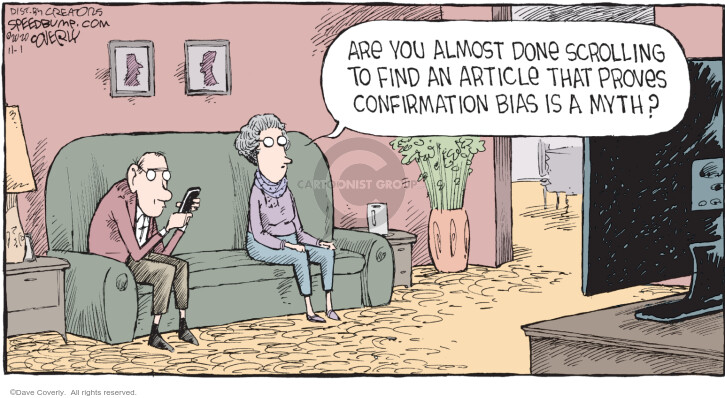
\includegraphics[height = .6\textheight]{ConfirmationBias.jpg}

}

%%%%%%%%%%%%%%%%%%%%%%%%%%%%%%%%%%%%%%%%%%%%%%%%%%%%%%%%%%%%%%%%%%
\frame{\frametitle{Desirability Bias}

\begin{block}{}
We prefer evidence that supports a conclusion we want to be true and discount evidence that undermines that conclusion.
\end{block}
~\\
\centering
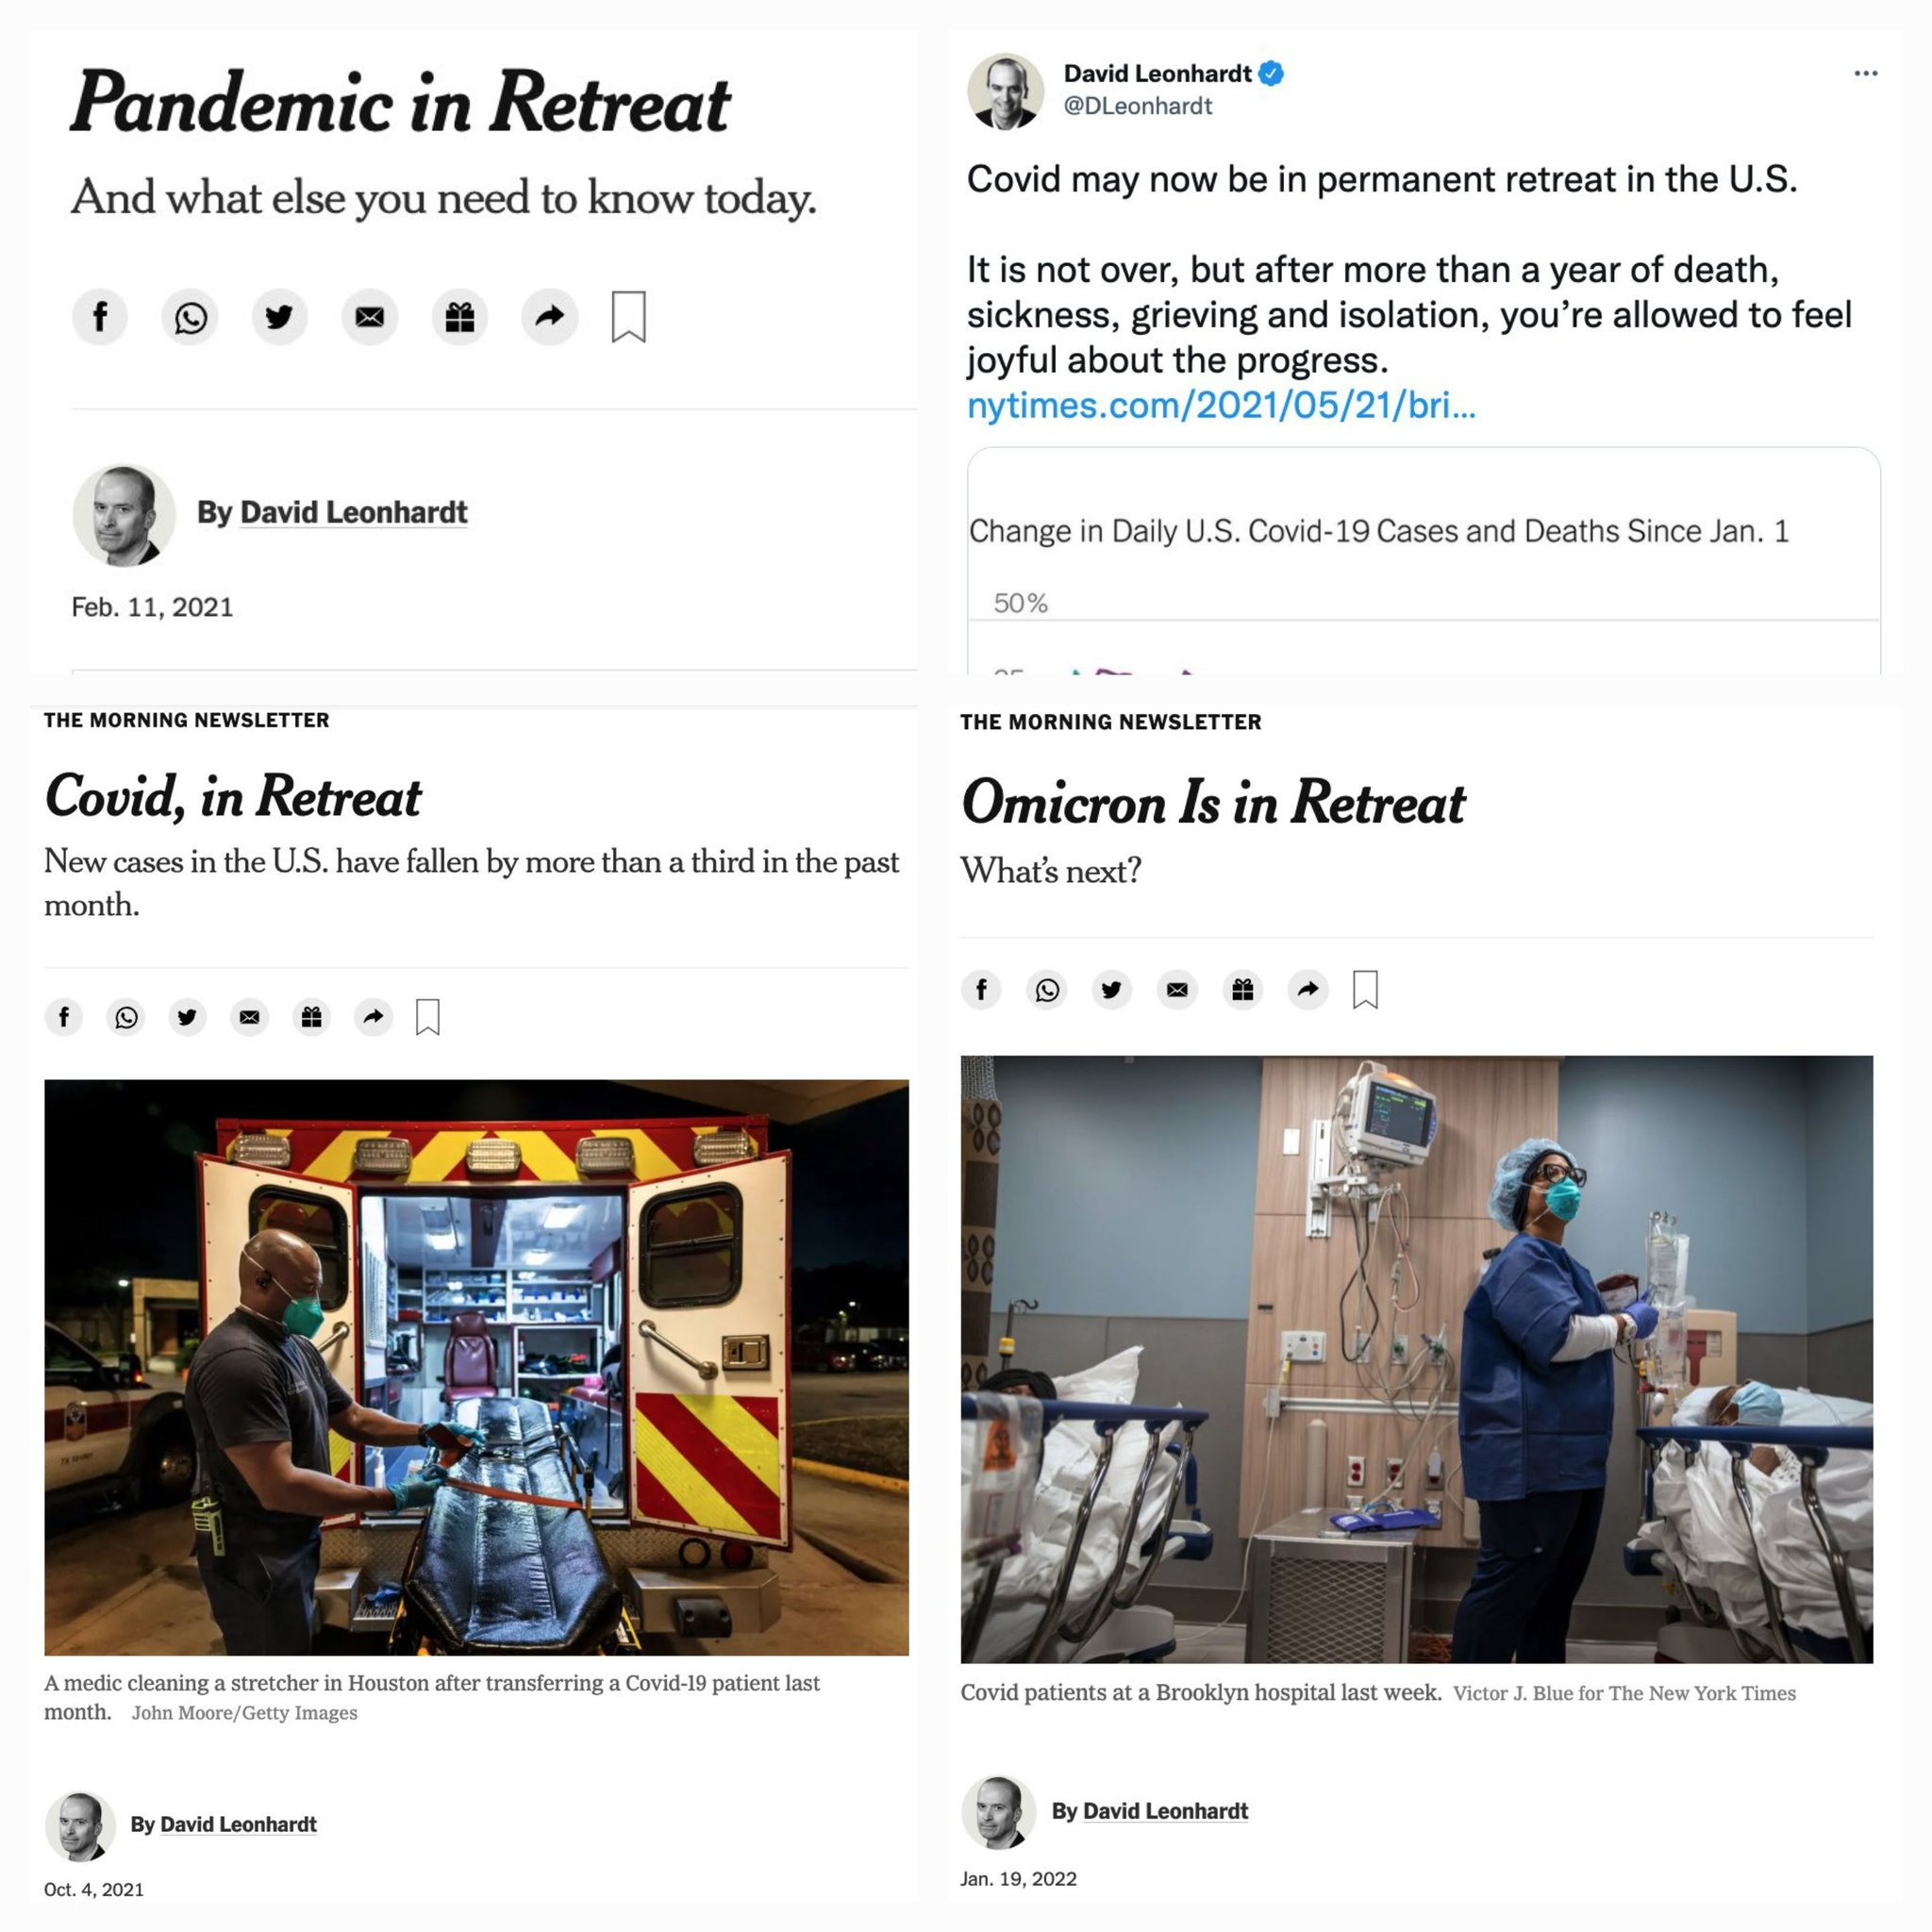
\includegraphics[height = .6\textheight]{Leonhardt.jpg}

}

%%%%%%%%%%%%%%%%%%%%%%%%%%%%%%%%%%%%%%%%%%%%%%%%%%%%%%%%%%%%%%%%%%
\frame{\frametitle{Authority Bias}

\begin{block}{}
We give greater weight to evidence offered by people in positions of authority.
\end{block}
~\\
\centering
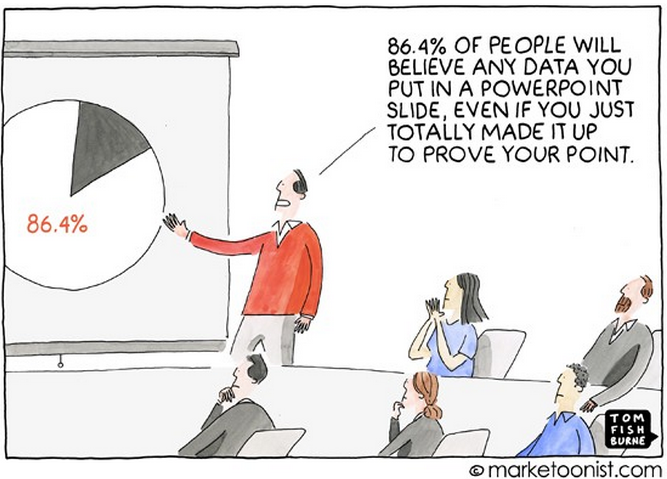
\includegraphics[height = .6\textheight]{AuthorityBias.png}

}

%%%%%%%%%%%%%%%%%%%%%%%%%%%%%%%%%%%%%%%%%%%%%%%%%%%%%%%%%%%%%%%%%%
\frame{\frametitle{Availability Bias}

\begin{block}{}
We give greater weight to evidence that is most memorable.
\end{block}
~\\
\centering
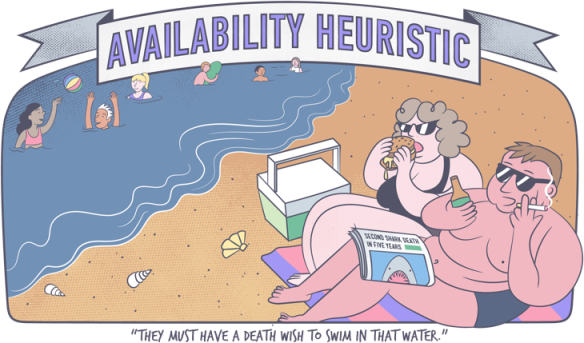
\includegraphics[height = .6\textheight]{AvailabilityBias.png}

}

%%%%%%%%%%%%%%%%%%%%%%%%%%%%%%%%%%%%%%%%%%%%%%%%%%%%%%%%%%%%%%%%%%
\frame{\frametitle{Certainty Bias}

\begin{block}{}
We over- and under-state probabilistic evidence.
\end{block}
~\\
\centering
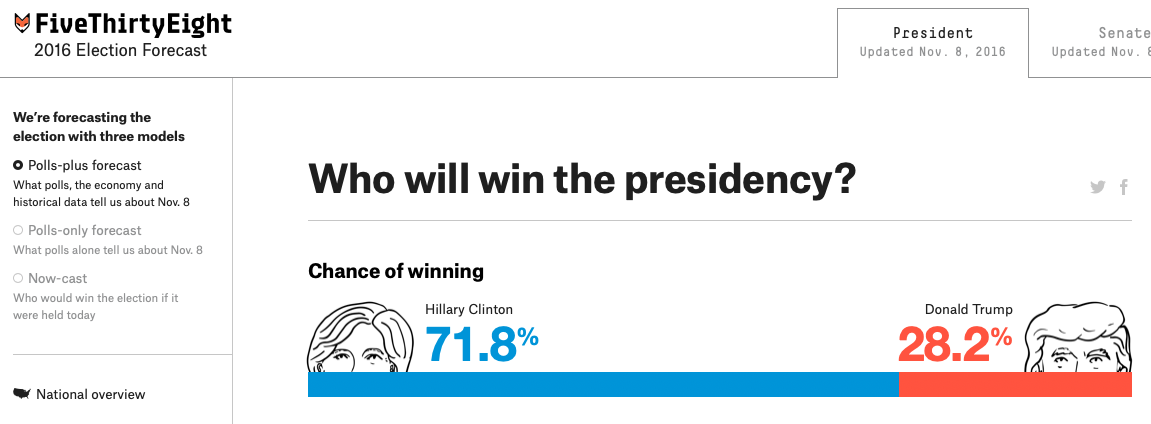
\includegraphics[width = .9\textwidth]{538_2016ElectionForecast.png}

}

%%%%%%%%%%%%%%%%%%%%%%%%%%%%%%%%%%%%%%%%%%%%%%%%%%%%%%%%%%%%%%%%%%
\frame{\frametitle{Retro Report (2021) - What's In a Number?}

\centering
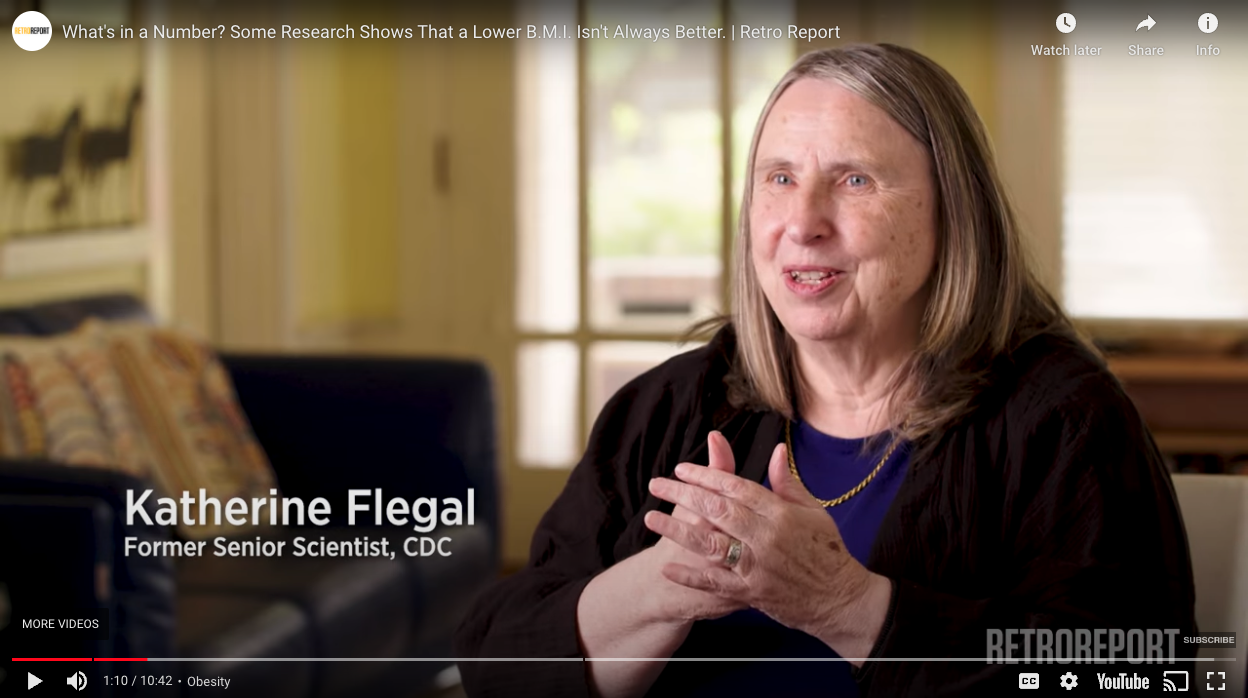
\includegraphics[width = .9\textwidth]{retro_report.png}

}

%%%%%%%%%%%%%%%%%%%%%%%%%%%%%%%%%%%%%%%%%%%%%%%%%%%%%%%%%%%%%%%%%%
\frame{\frametitle{Fraudulent Research}
\only<1-2, 10->{
    \begin{itemize}[<+->]
        \item Unfortunately, fraud does happen - perhaps more than researchers would like to admit
        \item One of the most infamous cases of fraud was a \href{https://www.youtube.com/watch?v=d8uRYqsu2W4}{study linking the childhood MMR (mumps, measles, and rubella) vaccine to autism}
        \item<10-> Red flags:
        \begin{itemize}
            \item<10-> Not sharing data or methods
            \item<11-> Unusual patterns in the data
            \item<12-> Non-reproducible outcomes or outcomes not supported by theory
            \item<13-> Conflicts of interest
        \end{itemize}
        \item<14-> These ``red flags'' do not necessarily mean the data is fraudulent -- but be vigilant
    \end{itemize}
}

\only<3-6>{
    \centering
    \textbf{Gay Canvassers Scandal}\\
    ~\\
    \includegraphics<3>[width = .8\textwidth]{lacour_result.png}
    \includegraphics<4>[width = .8\textwidth]{lacour1.png}
    \includegraphics<5>[width = .8\textwidth]{lacour2.png}
    \includegraphics<6>[width = .8\textwidth]{lacour3.png}
    }

\only<7-9>{
    \centering
    \small{\textbf{Dishonesty in Dishonesty Research (uncovered by Data Colada)}}\\
    ~\\
    \includegraphics<7>[width = .8\textwidth]{colada1.png}
    \includegraphics<8>[width = .8\textwidth]{colada2.png}
    \includegraphics<9>[width = .8\textwidth]{colada3.png}
    }
}

\end{document}
